%%% template.tex
%%%
%%% This LaTeX source document can be used as the basis for your technical
%%% paper or abstract. Regardless of the length of your document, the commands
%%% are all the same.
%%%
%%% The "\documentclass" command is the first command in your file. If you want to
%%% prepare a version of your article with line numbers - a "review" version -
%%% include the "review" parameter:
%%%    \documentclass[review]{acmsiggraph}
%%%

\documentclass[review]{acmsiggraph}

\usepackage{lineno}
\usepackage{float}
\usepackage{multirow}
\usepackage{array}
% \usepackage{units}
% \usepackage{color}

\usepackage{wrapfig}
\usepackage{tabulary}
\usepackage{amsmath} % assumes amsmath package installed
\usepackage{amssymb}  % assumes amsmath package installed
\usepackage{algorithm}
\usepackage[noend]{algpseudocode}



\algdef{SE}[DOWHILE]{Do}{doWhile}{\algorithmicdo}[1]{\algorithmicwhile\ #1}%


\newcommand{\todo}[1]{\textcolor{red}{TODO: #1}}

%%% Title of your article or abstract.

\title{Participatory Architectural Design and Fabrication\\
with Natural Materials in Native Forms
}

\author{Hironori Yoshida\thanks{e-mail:hyoshida@hy-ma.com}   Takeo Igarashi\thanks{e-mail:takeo@acm.com}, Maria K Larsson, Masaaki Miki
 \\www.hy-ma.com, the University of Tokyo
}



\pdfauthor{Hironori Yoshida}

%%% Used by the ``review'' variation; the online ID will be printed on
%%% every page of the content.

\TOGonlineid{0542}

% User-generated keywords.

\keywords{Fabrication, Collaborative Design, Human computation}

% With the "\setcopyright" command the appropriate rights management text will be added
% to your document.

%\setcopyright{none}
%\setcopyright{acmcopyright}
%\setcopyright{acmlicensed}
\setcopyright{rightsretained}
%\setcopyright{usgov}
%\setcopyright{usgovmixed}
%\setcopyright{cagov}
%\setcopyright{cagovmixed}
%\setcopyright{rightsretained}

% The year of publication in the "\copyrightyear" command.

\copyrightyear{2016}

%%% Conference information, from the completed rights management form.
%%% The "\conferenceinfo" command has two parameters:
%%%    - conference name
%%%    - conference date and location
%%% The "\isbn" field includes the year and month after the article ISBN.

\conferenceinfo{SIGGRAPH 2016 Posters}{July 24-28, 2016, Anaheim, CA}
\isbn{978-1-4503-ABCD-E/16/07}
\doi{http://doi.acm.org/10.1145/9999997.9999999}

\begin{document}

%%% This is the ``teaser'' command, which puts an figure, centered, below
%%% the title and author information, and above the body of the content.

\teaser{
    \centerline{
       \includegraphics[height=0.225\paperheight]{images/fabrication/teaser1.png}
       \hspace{3mm}
         \includegraphics[height = 0.225\paperheight]{images/fabrication/teaser3.png}
 }
  \caption{Left: an overview of the workflow: 1. fix branches on plates. 2. scan the plates and upload the model. 3. play the game with scanned branches. 4. fabricate joineries by a CNC (Computer Numerical Control) router. Right top: branch layouts designed using the game. 6 and 7 were designed and fabricated by participants in the case study. Right bottom: the fabricated 2D fence (2000 $mm$ $\times$ 900 $mm$). Each pair of branches is connected with rigid lapped joint. }

  \label{fig:teaser}
}


\maketitle

\begin{abstract}
Diverse natural materials such as stones and woods have been used as architectural elements since primitive shelters, however, the use of them in modern buildings is limited, mainly due to the irregular properties of non-standard materials.
In this paper, we take the diversity as playful inputs for design task, and present our game based design and fabrication platform for non-experts.
Taking tree branches as case study of non-standard found materials, our online game \textit{BranchConnect} enables users to design 2D networks of branches and realize the design with parametrically generated joineries.
As the generated design is realizable with ordinal 3-axis CNC milling machines, each connection has a customized unique joinery adapted to the diverse branch shapes.
The scoring system of the game guides users to design structurally sounding solutions with given branches.
Together with low-cost mobile scanning devices, everyone can contribute to design and fabrication process not only as a game user, but also from collecting branches around their physical environments and uploading them to our online platform.
For validating our process, we conducted a workshop with non-experts, and let them collect branches in a nearby forest, and design/fabricate a 2D fence by integrating multiple design solutions.
\end{abstract}

\linenumbers

%
% The code below should be generated by the tool at
% http://dl.acm.org/ccs.cfm
% Please copy and paste the code instead of the example below.
%
\begin{CCSXML}
<ccs2012>
<concept>
<concept_id>10010147.10010371.10010382</concept_id>
<concept_desc>Computing methodologies~Image manipulation</concept_desc>
<concept_significance>500</concept_significance>
</concept>
<concept>
<concept_id>10010147.10010371.10010382.10010236</concept_id>
<concept_desc>Computing methodologies~Computational photography</concept_desc>
<concept_significance>300</concept_significance>
</concept>
</ccs2012>
\end{CCSXML}

\ccsdesc[500]{Computing methodologies~Image manipulation}
\ccsdesc[300]{Computing methodologies~Computational photography}

\keywordlist

\conceptlist

\printcopyright

\section{Introduction}
Modern buildings are characterized by its uniformity; built upon the same principle of construction system, consisting of standardized building component and its assembly process.
The standardized construction system is favored because of its efficiency in design and production.
As each component satisfies specified structural performance, the resulting structure can be analyzed systematically.
On the other hand, the excessive standardization caused generic designs of architecture which are criticized for being detached from local culture ~\cite[frampton1997towards].
Reacting on the issue, designers and architects actively use local materials not only as inspirational sources, but also as a catalyst of their design to the local context \cite{oliver1997encyclopedia}.

% As a result, we see similar-looking buildings all over the world.
%The aesthetic quality of the combination of construction techniques to deal with building components is described as "techtonik".
% Including management of construction, guidelines for maintenance to building materials and construction techniques, we call it as building starndard.
Since primitive shelters and huts, traditional construction has used locally found natural materials directly in their native forms \cite{weston2003materials}.
Such a direct use can not compete with highly standardized materials and construction system, however, the uniqueness of native forms is a valuable quality which is lacking in standardized materials.
As the material is locally obtained, building and living get much closer, thus people using the building can easily commit design and fabrication, fostering the sense of belonging to the community.
Locally obtained materials can easily connect design and the context of built environment in this way, but their irregular properties limit the use of them in modern buildings.
Traditionally, craftsman has taken care irregular natural materials varying their native forms and dynamically design the global design by considering individual material properties \cite{pye1968nature}.
Such a task is difficult to be automated and these skills are developed through years of training, thus the use of native forms typically inaccessible for end users and costs more than standardized construction system. \\

This paper aims to make the above-mentioned qualities of materials in native forms more accessible for end users by leveraging digital technologies.
We use locally obtained branches which can be found almost everywhere not only in countryside but also in urban environment such as parks and along streets.
Public service takes care of these branches: annual pruning, storing, and chipping or burning with some costs.
The size of branches (from 50 -300 $mm$ in diameter) is too small for furniture or other structural applications as building components.
It is a challenge for digital design and fabrication to utilize the diverse branches in meaningful ways.
High-precision but low-cost scanning devices and personal digital fabrication machines make it possible to analyze and control natural materials in diverse native forms.

The key technical difficulty of materials with natives forms is design.
A possible approach is optimization: minimize an energy function which integrates structural and fabrication costs.
This approach, however, is limited to particular design scenario with specific materials.
Furthermore, the concept of optimum solution is well suited to goals such as efficiency or low-cost, but these goals are not the qualities materials in natives forms can compete with standardized construction systems.
Instead, we take humans in our scan-design-fabricate workflow not only to solve the design problem, but also to provide an opportunity for people to participate in the workflow.
Traditionally, in case of constructing public and symbolic buildings, such as church, people in a community took initiatives from fund raising to design, or even in construction process.
% In this way, our method would be applicable to other kinds of materials with diverse shapes.

% The humans-in-the-loop also enrich the connection between users and a building.
% put emphasis on the forementioned qualities such as diverse solutions not only from the native diverse shapes but also from multiple solutions by people living and using the local community.
% In modern architecture, user partricipation in design has been commonly explored for enhancing connection between the design and the context as a reaction against the generic buildings.

%Historically, local natural stones and wavy trees have been commonly used to construct primitive huts and shelters \cite{weston2003materials}.
% Over the years, each unique solution has been converged into a symbolic building style per community, described as "vernacular" in architecture


In this paper, we report our case study to design and fabricate an architectural element out of irregularly shaped branches, using our humans-in-the-loop system.
We developed an online platform where users can post branches found at hand, and design with them through the online game \textit{BranchConnect} \footnote{Please visit and play the game. \url{https://branchconnect.herokuapp.com/start}}.
The game system itself helps users to design feasible branch layouts and enable them to fabricate customized joints to connect them together without screws and adhesives.
The design of our joint extends the traditional orthogonal lap-joints to various angles within a range, freeing the diverse forms of woods from orthogonal connections.
Physically collected branches are digitally scanned and stored in a cloud database \textit{BranchCollect}, and offline application \textit{Branch Importer} analyzes forms of branches and upload them to the database.
The simple visual feedback and scoring system of the game guide users to feasible solutions, which are further inspected by an offline application \textit{G-Code\footnote{G-Code is the generic name for a control language for CNC machines.} Generator} for CNC milling process.
The game system and developed import/export applications are currently limited to branches, however, the principle of human-in-the-loop with design is applicable for other kinds of materials with diverse irregular forms.
We hope our method sheds lights on materials such as waste from demolition of buildings for various design applications.

% but selected  as well as fabricating differentiated joints by a CNC router.
% We propose an accessible design and fabrication platform, which allows multiple users to design with diverse irrefular forms of branches.

In summary, our contributions are
\begin{itemize}
 \item{a workflow enabling to take natural materials in native forms as design components.}
 \item{an online game-based approach to participatory architectural design and fabrication.}
 \item{a method to design and fabricate customized non-orthogonal joints using high-resolution contours.}
\end{itemize}



% First of all, non-standard materials are considered to be expensive and less performative compared to standardized building materials.
% For example, fabricating wooden joints is considered to be an art due to the heterogeneous wooden structure and its precisions, resulting in higher cost than repetitive assembly of standard components \cite{seike1977art}.
% In the context of fabrication, Pye \shortcite{pye1968nature} described such a skill as ``\textit{workmanship with risks}'', in contrast to ``\textit{workmanship with certainty}''.
% Due to the complexity, these skills are not fully automated yet, thus we rely on skilled-workers to design and fabricate with these diverse materials.
% Second of all, building design and construction became highly specialized professions.
% Not only skills and knowledge, but also designers and architects must communicate with local municiparity to clear legal building codes.
% Although participatory design has been common in architectural design process, the degree of participation is limited.
% There is no such a platform to include local community to design and construction.

% In this project, we put emphasis not only on sustainable, economical aspects of architecture, but also on cultural, communal aspects.
% With the digital technology, we make the design process accessible for users by online browser game.
% The approach is similar to participatory design process in architecture.
% We believe that the use of non-standard materials provides an alternative design approach to modern architectural design.
% As a prospect, we also aim to reveal implicit knowledge to handle such non-standard materials, which has been fostered in craftsmanship.

\section{Related Work}
3D printers and CNC routers made digital fabrication more accessible, and pre-fabricated customized parts are often used in buildings nowadays \cite{knaack2012prefabricated}.
According to Pye, these parts are processed from highly standardized material, thus its digital fabrication process is ``workmanship with certainty''; a batch process of reading G-Code and strict execution of the code.
On the other hand, as ``workmanship with risks'' with digital technologies, interactive fabrication enables machines to pick up uncertain happenings and react on it \cite{willis2011interactive}.
Mueller developed interactive laser cutting, taking user inputs and recognizing placed objects in a fabrication scene \cite{Mueller:2012:ICI:2380116.2380191}.
While their system interprets objects as simple platonic geometry, our work takes the branches with diverse shapes.
While Crowdsourced fabrication project took advantage of humans-in-the-loop in their fabrication system \cite{lafreniere2016crowdsourced}, our work puts emphasis on crowd-sourced design.
As a crowd-sourced design system, Jerry et. al., developed a platform for light users to design trees and plants \cite{talton2009exploratory}.
Our design process is not parametric modeling, also directly linked to physical world. \todo{ill-logic}

There are few works that take natural materials with native shapes as design components.
Schindler and his colleagues used digitally scanned wood branches and used them for furniture and interior design elements \cite{schindler2014processing}.
Monier and colleagues virtually generated irregularly shaped branch-like components and explored designs of large scale structure ~\cite{monier2013use}.
Using larger shaped forked tree trunks, \textit{Wood Barn} project designed and fabricated custom joineries to construct a truss-like structure\cite{woodbarn}.
\textit{Smart Scrap} project digitally measured lime stone leftover slates from a quarry and digitally generated assembly pattern of slates \cite{smartscrap}.\\

In industry, recognition of irregularly shaped objects is essential for waste management.
\textit{ZenRobotics} developed a system that sorts construction and demolition waste by picking objects on a conveyor belt using robotic hands \cite{lukka2014zenrobotics}.
For factory automation purpose, there is a system that recognizes irregularly shaped objects and sort them into a container \cite{sujan2000design}.
Getting out from factories, autonomous robotics in construction site is a hot topic among roboticists \cite{feng2014towards}.
\textit{In-situ Fabricator} is a system which could be installed in construction site and co-operated with human workers \cite{dorfler2016mobile}.
Once robot is autonomously localize itself in such an environment, it can build foundational structure for further construction \cite{napp2014distributed}.
Using locally found objects on-site, such a system can be much simpler.\\

While these projects demonstrated the capability of digital fabrication processes to handle irregularly shaped materials, design process is still dependent on a designer or architect who has experiences with materials or has access to special software.

Cimerman discussed architectural design practices that took computer-mediated participatory design \cite{cimerman2000participatory}.
He mentioned three motivations of digital participatory design:
\begin{itemize}
 \item{Including stakeholders in creation of one's environment.}
 \item{Experimenting diverse design tastes from multiple point of views.}
 \item{Solving complex design tasks with full of diverse solutions.}
\end{itemize}
Opening database of available local materials, people with various backgrounds can involve in design process, which could lower the cost of design fee with natural materials with native shapes.
For example, \textit{Nano-Doc} took gamification approach to search valid nano-particle designs against tumors out of infinite design space \cite{hauertcrowdsourcing}.
\textit{DrawAFriend} has developed an online game to collect big-data for drawing applications which assist humans with auto-stroke assistance \cite{limpaecher2013real}.
While these works developed games which are collecting data for solving medical or engineering problems, our game intends to provide a participatory design platform as a solution for social and cultural problems context-aware architectural design with locally found natural materials.
 \todo{ambiguous!}

\section{Workflow}
% As shown in Figure \ref{fig:teaser} left, our workflow starts from physically collecting branches.
In this section, we introduce two steps in the workflow shown in \ref{fig:teaser} left: Collecting and Scanning Branches (1 amd 2 in Figure~\ref{fig:teaser} left) and Fabrication (4 in Figure~\ref{fig:teaser} left).
As for the game (3 in Figure~\ref{fig:teaser} left), please refer Section \ref{sec:game}.
The collected branches are uploaded to cloud database by \textit{Branch Importer}, and served to the online game-based design application \textit{BranchConnect}.
The game system uses skeletons for its joint detection process, which works on browsers on laptop computers or mobile touch devices.
As shown in Figure \ref{fig:teaser} right, users can explore a global design with various layouts designed by multiple users.
Once layouts for each frame are selected for completing a global design, these layouts are further inspected by \textit{G-Code Generator}, which generates customized joints for CNC milling.
After finishing the milling process, users physically assemble branches and complete the fabrication process.
The pipeline of the workflow is illustrated in the Figure \ref{fig:pipeline}.

\begin{figure}[ht]
  \begin{center}
    \includegraphics[width = 0.4\paperwidth]{images/workflow/pipeline.png}
    \caption{A pipeline from model acquisition to fabrication.}
    \label{fig:pipeline}
  \end{center}
\end{figure}

\subsection{Collecting and Scanning Branches}
Users can collect branches and upload to the online database.
Considering the mechanical constraints of CNC milling machine, branches are cut in certain length.
The cut branches need to be firmly fixed to plates for milling process.
We use metal fixtures to attach them on a plate (See Figure~\ref{fig:skeleton}).
After attaching branches on plates, users can start scanning and acquire textured mesh model.
For more details of preparation of branches and scanning setup, please refer Section~\ref{sec:user_experiences} for details.
%As complete mesh model provides more robust results with 3D shapes of branches, we describe our process based on mesh model as an input.
Taking mesh model with colored texture, our \textit{Branch Importer} provides functions such as object detection, skeleton extraction, branch type classification, and fixture point setting.
The scanned result is a mesh model representing branches with a base plate.
The system first identifies branches by applying simple height threshold, and then applies contour detection.
The obtained 2D contours are used for extracting skeletons and clustering vertices in the mesh model.
Contours are triangulated and skeleton points are extracted from middle points on edges of triangles.
These middle points are compared with top view image.
If the point is inside of a contour, the middle point is counted as a skeleton point.
After extracting skeleton points, the connectivity of skeletons is analyzed.
In case grafting branch (Y-shaped branch) is detected, a new skeleton sub-branch is added.
The result is shown in Figure ~\ref{fig:skeleton}.
%Evaluating the number of sub-branches, the branch is morphologically classified.
Metal fixture locations are confirmed by simple mouse-clicks and marked as invalid, meaning that joints should not be placed on these points.
The acquired information is stored in a cloud database.

\begin{figure}[ht]
  \includegraphics[width = 0.4\paperwidth]{images/importer/importer_2.png}
  \caption{An interface of \textit{Branch Importer}. Left: a top ortho-view image of textured mesh model. The model also shows the metal fixtures where joints can not be generated. Right: Extracted skeletons are shown with blue dots. The beginning of skeletons is shown bigger dots, and the red dots are invalid points defined by a user. }
  \label{fig:skeleton}
\end{figure}


\subsection{Fabrication}
\label{sec:fabrication}
After a design is selected for fabrication, fabricatability of the design is further inspected by a high-resolution model.
The \textit{G-Code Generator} displays joints and milling paths on scanned orientations.
If it identifies an invalid joint in the high resolution model, a layout can be easily modified with simple mouse inputs (Figure \ref{fig:joint_geometry}.1 and \ref{fig:joint_geometry}.2).
Users can also change milling parameters such as offset ratio of milling paths, milling bit diameter, depth of joints, cutting speed, moving height and so forth.
After confirming the fabrication settings and milling paths, it generates G-Code.\\

Some fabrication factors such as invalid points due to metal fixtures and flipped (further described in Section \ref{sec:joint}) are already considered by \textit{Branch Importer} and the game system respectively.
Here, we describe the process to calculate joint geometry for fabrication.
The \textit{G-Code Generator} searches a set of four closest points on high-resolution contours (Figure \ref{fig:joint_geometry}.1).
By trimming contours of each branch at the corner points, we get \textit{side cuts} and \textit{center cuts} (Figure \ref{fig:joint_geometry}.4).
% Please refer Appendix~\ref{sec:sidecut} for details of this process.
\textit{Side cuts} have wedged corners for smooth assembly process.
The depth of the \textit{center cuts} is half of the top height at the joint position from a mesh model (Figure \ref{fig:joint_geometry}.4).
The bottom height is usually the height of the base plate, however, in case of under-cuts with incomplete mesh model, we calculate a half of the diameter from the 2D contour and subtract it from the top height.
The resulting geometry creates rigid joints with irregularly shaped sections.

\begin{figure}[h]
	\begin{center}
		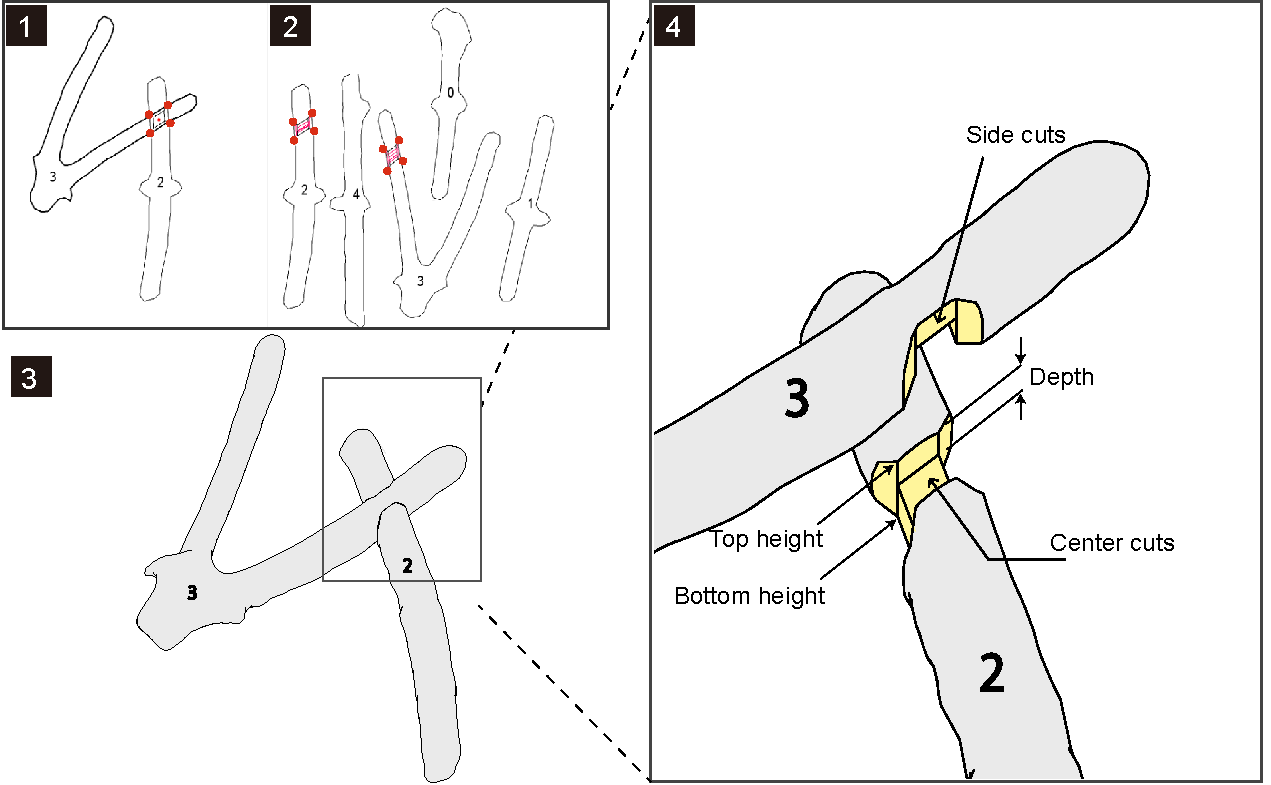
\includegraphics[width = 0.4\paperwidth]{images/system/joint_diagram.pdf}
		\caption{1, 2: an interface of G-Code Generator. 1. a layout defined by a user. 2. the original orientations of branches with generated milling paths with red color. 3. an assembled pair of branches with branch 3 is flipped. 4. milled branches with center cuts and side cuts.}
		\label{fig:joint_geometry}
	\end{center}
\end{figure}

\section{Workflow}
As illustrated in the left of Figure \ref{fig:teaser}, our workflow starts from physically collecting branches.
The collected branches are uploaded to cloud database by \textit{Branch Importer}, and served to online game-based design application \textit{BranchConnect}.
The game is working on browsers and accessible from laptop computers and mobile devices.
As in the right of \ref{fig:teaser}, users can explore a global design with multiple branch layouts.
Once the global design is fixed, designed layouts are further inspected by \textit{G-Code Generator}, which generates customized joineries for CNC milling.
After finishing the milling process, users physically assemble branches and complete the fabrication process.
The pipeline of the workflow is illustrated in the Figure \ref{fig:pipeline}.
In this section, we describe three steps in the pipeline: Digital Model Acquisition, the Game System, and Fabrication.

\begin{figure}[ht]
  \begin{center}
    \includegraphics[width = 0.4\paperwidth]{images/workflow/pipeline.png}
    \caption{A pipeline from model acquisition to fabrication.}
    \label{fig:pipeline}
  \end{center}
\end{figure}

\subsection{Digital Model Acquisition}
Our system takes textured mesh model or point cloud with colored vertices.
As complete mesh model provides more robust results with 3D shapes of branches, we describe our process based on mesh model as an input.
There are various methods and software available for scanning 3D models.
As for scanning setup, we describe in the Section \ref{sec:casestudy}.
Taking mesh model with colored texture, our \textit{Branch Importer} provides functions such as object detection, skeleton extraction, branch type classification, and fixture point setting.

The scanned result is a mesh model representing branches with a fixed plate.
The system first idendifies branches by applying simple height threshold, and then applies contour detection (we currently use \textit{findContour} in OpenCV \footnote{Open Source Computer Vision Library: \url{http://opencv.org/} }).
The obtained 2D contours are used for extracting skeletons and clustering point cloud in the mesh model.
Contours are triangulated and skeleton points are extracted from middle points on edges of triangles.
These middle points are compared with top view image from OpenCV.
If the point is inside of a contour, the middle point is counted as a valid point.
After extracting valid middle points, the connectivity of skeletons is analyzed. 
In case grafting branch is detected, a new skeleton sub-branch is added. 
The result is shown in Figure ~\ref{fig:skeleton}.
%Evaluating the number of sub-branches, the branch is morphologically classified.
Metal fixture locations are confirmed by simple mouse-clicks and set as invalid points.
The acquired information is stored in a cloud database.

\begin{figure}[ht]
  \includegraphics[width = 0.4\paperwidth]{images/importer/importer.png}
  \caption{An interface of \textit{Branch Importer}. Left: a top ortho-view image of textured mesh model. Right: Extracted skeletons are shown with blue dots. The beginning of skeletons is shown bigger dots, and the red dots are invalid points defined by a user. }
  \label{fig:skeleton}
\end{figure}


\subsection{BranchConnect: The Game}
The online game is accessible by laptops and mobile touch devices, and many users can play at the same time.
The objective of the game is to collect valid layouts of branches which are fabricatable with 3 axis CNC milling machines.
By analyzing the connectivity of branches and target points, the game checks structural feasibility of a given layout. 
The guidance system during furniture design inspected connectivity, durability, and stability \cite{umetani2012guided}. 
Unlike their work, our game focuses on fabricatability with minimum consideration of gemetric connectivity due to the limited resources with mobile devices.


%The workflow of the game is illustrated in Figure~\ref{fig:game_flowchart}.
%\begin{figure}[ht]
%  \begin{center}
%    \includegraphics[width = 0.25\paperwidth]{images/system/systemFlowChart.pdf}
%    \caption{The workflow of \textit{BranchConnect}. Branch data and user design data are stored on cloud database.}
%    \label{fig:game_flowchart}
%  \end{center}
%\end{figure}

Firstly a user selects a frame indicating multiple target points to be connected, and then selects a set of branches fixed on a plate (The left in Figure \ref{fig:game_interface} ).
After selecting the target frame and the set of branches, the user is guided to the game interface, consisting of the frame with the target points, and the set of available branches (The right in Figure \ref{fig:game_interface} ).
The user picks a branch from the available set on the bottom, and then places it in an arbitrary 2D pose through basic manipulations such as move, rotate, and mirror.
The number of available branches differs depending on plates.
With the feasible diameter of branches (over 2cm) and the plate size (50cm x 50cm), the number of available branches is most likely up to six.
Within the limited number of branches, the user bridges all the target points by connecting all the used branches in one group.
The game is completed when all the target points are connected.
For higher score, the user can modify the design after the completion, and save it to the database.

\begin{figure}[H]
  \begin{center}
    \includegraphics[width = 0.4\paperwidth]{images/interface/game_interface.png}
    \caption{Left: the selection interface for target frames (top) and branch panels (bottom). Right: the start interface of the game.}
    \label{fig:game_interface}
  \end{center}
\end{figure}
%
\subsubsection*{System Overview}
There are many collision detection libraries available, however, our game needs to detect intersected branch pairs, thus surface contact detection is overkill for our application.
Also most branches come with free-form concave shapes, thus further geometric preparation such as convex decomposition is necessary for using these libraries.
For fast and robust intersection detection, our system extensively uses skeletons of branches.

Hubbard and Philip developed collision detection by representing object with hierarchical 3D spheres aligned on skeletons \cite{Hubbard:1996:APS:231731.231732}.
Our system takes similar approach but limited in 2D, but more focused on searching fabricatable joints.
In the game, simplified skeletons are used to find the pair of closest skeleton points between two branches.
When a branch is selected, it is counted as an active, and the system searches the closest skeleton point from skeletons of other branches.
More precise joint calculation with higher resolution is further described in the next section.

A joint is created when an intersecting pair is detected, and the pair forms a group.
The group is used for evaluating connections between target points (\textit{Bridged}).
The game is completed once all the target points are connected by a group of branches.
The conditions of joint and group are indicated with simple color-code.
Once the user finishes positioning, score is updated with weighted sum of parameters.
Together with the color-code, the score update guides the user to form a valid design.


\subsubsection*{Joint Condition}
Joint is the essential entity not only in the game but also in the fabrication process of customized lapped joineries.
Each fabricated joint works as a rigid joint, and we do not calculate structural performance of each joint.
Figure~\ref{fig:joint_condition} illustrates valid and invalid joint conditions.
Our joint only takes crossed pair (see Figure~\ref{fig:joint_condition}.1) because they are structurally stable, relatively simple to fabricate, and creates diverse designs. 
Tangential connections are counted as invalid as fabrication of tangential joinery is challenging with small branches (see Figure~\ref{fig:joint_condition}.3).

\begin{figure}[ht]
	\begin{center}
		\includegraphics[width = 0.4\paperwidth]{images/system/joint_conditions_2.png}
		\caption{Joint conditions. 1.valid joint. 2.invalid for violating the angle. 3.invalid tangential connection. 4.invalid for connecting on a fixture point. }
		\label{fig:joint_condition}
	\end{center}
\end{figure}


A valid joint's angle stays within a fixed range (see Figure~\ref{fig:joint_condition}.1 and 2). 
Joints close to metal fixtures are also counted as invalid (see Figure~\ref{fig:joint_condition}.4).
Valid and invalid joints are displayed with green and red respectively.
When a branch is connected to a target point, the specially added score is deisplayed in a pop-up square, also the graphics of target point's and the branch are changed.
The branch is trimmed at the connection point with the target point, and the trimmed length is subtracted from the score.

To describe the process, we let $\mathcal{B}$ denotes a set of all the available branches, and each branch as $ b_i \in \mathcal{B}$.
While the process checks joint condition through all the branches $\mathcal{B}$, each detected joint is stored in each branch $b_i$, categorized in different conditions such as valid and invalid joints denoted as $j_{\text{valid}, j, i} \in \mathcal{J}_{\text{valid},i}$ and $j_{\text{invalid}, j, i} \in \mathcal{J}_{\text{invalid},i}$ respectively.
When a branch $b_i$ is connected to one of target point $t_j \in \mathcal{T} $, the $t_j$ is stored in $b_i$.


A flowchart of the game system with joint and group conditions is illustrated in Figure \ref{fig:system_flowchart}.

\begin{figure}[ht]
	\begin{center}
		\includegraphics[width = 0.35\paperwidth]{images/system/closestPointAlgorithm.pdf}
		\caption{Left: an overview of the game system with 1.joint checkand 2.group check and 3. score calculation. This process is iteratively executed while a user is exploring layout by dragging a branch. The joint check process is further illustrated in the right, and group condition check is described in Algorithm \ref{al:connection}. }
		\label{fig:system_flowchart}
	\end{center}
\end{figure}

% well as the paired branch $b_{\text{paired},j} \in \mathcal{P}_{\text{paired},i}}$.



\subsubsection*{Group Condition}

After checking joint conditions of all the pairs of branches, the system checks the number of groups as well as its connection with the target points on a frame.
If a group is not connected to any target point nor other groups, the group is \textit{Islanded} and structurally invalid.
While a user is positioning a branch by dragging or rotating, groups are continuously calculated and indicated by simple color (Figure \ref{fig:group}).

\begin{figure}[ht]
  \begin{center}
    \includegraphics[width = 0.4\paperwidth]{images/interface/groups.jpg}
    \caption{Left: valid group with two target points connected. Middle: valid but three groups. Right: invalid due to the \textit{Islanded} situation. }
    \label{fig:group}
  \end{center}
\end{figure}


After all the joint conditions are checked, we evaluate group conditions.
Through checking the all the branches $\mathcal{B}$, the first group $g_0$ is created and stored as $b_0$.
%The other paired branch $b_{\text{paired},i}$ stored in $j_{\text{valid}, j}$ is used for tracing the connection with other paired branch in each valid joint $j_i$. \todo{incomplete sentence!}
The game is completed when the number of $\mathcal{G}$ is one, and all the target points are connected with the group.
The algorithm chekcing group conditions is described in \ref{al:connection}.

\begin{algorithm}
  \caption{Group Condition Update Algorithm}
  \begin{algorithmic}[1]
    \Function{UpdateGroups}{$\mathcal{B}$}
    \State{Reset all the groups $\mathcal{G}$ }
    \State{Create new group $g_0$}
    \State{$b_0 \text{ is added to } g_0$}
    \If{$b_0$ has connected target point $t_i \in \mathcal{T}$}
      \State{$g_0 \text{ sets } t_i$}
    \EndIf
    \State{$g_0 \text{ is added to }  \mathcal{G} $}

    \For{each branch $b_i$ in $\mathcal{B}$}
    \State{\textit{GroupConnection} $\gets false$}
      \For{each group $g_j$ in $\mathcal{G}$}
        \For{each branch $b_j$ in $g_j$}
          \If{ $b_{\text{paired},i} \in \mathcal{P_i}$ has $b_j$}
            \State{ $b_i  \text{ is added to } g_j $}
            \State{ \textit{GroupConnection}  $\gets true$}
            \If{($b_i$ has $t_i$) and ($g_j$ has $t_j$) }
              \State{ Set $g_j$ as \textit{Bridged}}
            \EndIf
            \If{$g_j$ has no $t_j$}
              \State{ Set $g_j$ as \textit{Islanded}}
            \EndIf
            \State {\textit{break}}
          \EndIf
        \EndFor
      \EndFor

      \If{ \textit{GroupConnection} is \textit{false} }
        \State{create new group $g_{new}$}
        \State{ $b_i  \text{ is added to } g_{new}$}
        \State{$g_{new} \text{ is added to }  \mathcal{G}$}
      \EndIf
    \EndFor

  \EndFunction
  \end{algorithmic}
  \label{al:connection}
\end{algorithm}

\subsubsection*{Score Calculation}
In the score calculation processes, follwoing entities forms the score: the numbers of valid and invalid joints on each branch, the number of groups as $N(\mathcal{G} )$, the number of islanded groups as $N(g_{\text{islanded}} \in \mathcal{G} )$, the number of bridged target points as $N(t_{\text{bridged}, i}) \in \mathcal{T} )$.
The trimmed lengths of branches which are connected with target points are denoted as $trimmed(t_j, b_i)$
The score is weighted sum of these joint and group conditions, denoted in Equation (\ref{eq:cost}).
The weights 'w1...w5' are non-negative weight coefficients pre-adjusted in advance by authors.




\begin{equation} \label{eq:cost}
 \begin{aligned}
 Score =  &\; w_1  \sum_{1}^{N(\mathcal{B})} \sum_{1}^{N(\mathcal{J}_{\text{valid},i})} j_{\text{valid}, j, i} 
	& + \; &w_2  \sum_{1}^{N(\mathcal{B})} \sum_{1}^{N(\mathcal{J}_{\text{invalid},i})} j_{\text{invalid}, j, i}\\
+ &\; w_3  \sum_{1}^{N(\mathcal{G})} g_{\text{islanded}} \;
	& + \; &w_4  \sum_{1}^{N(\mathcal{T})} t_{\text{bridged}} \; \\
+ &\; w_5 \sum_{1}^{N(\mathcal{T})} trimmed(t_j, b_i)
 \\
   \textrm{s.t.} \; w_j  \geq  &\;0 \; \forall j \in 1, \dotsc , 5 
 \end{aligned}
\end{equation}

\subsection{Fabrication}
After a design is selected for fabrication, the validity of the design is further inspected with a high-resolution model.
The \textit{G-Code Generator} was developed for fine-tuning the design by checking real-time feedback of updated joineries on branches with scanned orientations (see Figure \ref{fig:gcode_gen}).
Users can change fabrication parameters such as offset ratio for the side cuts, milling bit diameter, overlapping ratio for defining the center cut depth, feed-rate, moving height and so forth.
After confirming the fabrication settings and milling paths, it generates G-Code.

\begin{figure}[ht]
  \begin{center}
    \includegraphics[width = 0.4\paperwidth]{images/system/joint_generator_2.png}
    \caption{Interface of \textit{G-Code Generator}. Users can tweak the design on the left side and immediately see the updated joints and milling paths on the right. }
    \label{fig:gcode_gen}
  \end{center}
\end{figure}

Some fabrication factors such as mirror and invalid points are already considered by \textit{Branch Importer} and the game system.
In this section, we describe the process of joinery generation.
Each joinery geometry is parametrically modeled with: two plane surfaces on the sides of branches and one plane top surface (see Figure \ref{fig:joint_geometry}).
The geometry creates rigid connection with the irregularly shaped sections of branches.\\

Similar to the joint searching process with skeletons, the \textit{G-Code Generator} searches a set of four closest points from high-resolution contours, expecting that every intersected contour has four curves.
After finding the four closest points, it trims two curves from each contour of branch. (two from intersecting branch and two from intersected branch) at each joint.
The trimmed contours are transformed to the original scanned orientation and used for generating milling paths.
Two curves from an intersected branch are used for side cuts milling paths, which are inwardly offset paths of the original branch contours. 
The center cuts are paths that are plaining the top surface of the joint.
Height of center cuts is calculated with a diameter of cross-section at the center of a joint and the actual height information stored in point cloud. \todo{strange sentence}


\begin{figure}[ht]
  \begin{center}
    \includegraphics[width = 0.4\paperwidth]{images/system/joint_milling_diagram_4.png}
    \caption{An example of intersected pair: 1. an assembled pair of branches. 2. branches after the center and side cuts are milled 3. left: a layout defined by a user right: the original orientations of branches with generated milling paths with red color.  }
    \label{fig:joint_geometry}
  \end{center}
\end{figure}



\section{Case Study}
\label{sec:casestudy}
A design and fabrication workshop was organized to examine the feasibility of our system with a specific design target and a location.
Prior to the workshop, we have adjusted the weights in Equation \ref{eq:score} manually to ensure that the feasibility of layouts is correlating to the scores (Figure \ref{fig:testlayouts}).
Through adjusting the game setting, we have built six target frames.


We selected a public community house where people in the community share the space and regularly use the facility.
Participants of the workshop were selected among them, who were four children (aged 4, 7, 9, and 10) and two parents (Figure~\ref{fig:workshop}).
We specifically selected children with this range of age as non-experts without experiences in computational design or digital fabrication, also for observing the clarity and attractiveness of the game.
The entire workshop was filmed and summarized in the supplementary video material.
During the game play, we collected following data per click: frame count, click count, selected branch, and poses of all the branches at the click.


The goal for the participants was to contribute to an ongoing design and fabrication process of screen wall (2000 $mm$ $\times$ 900 $mm$) consisting of eight rectangles (500 $mm$ $\times$ 450 $mm$).
Six frames were already designed and built, thus the rest two frames (6 and 7 in Figure \ref{fig:teaser}) were assigned for them to design and fabricate in this workshop.

Participants were informed about the goal of the workshop, and each process was introduced and supervised by an author.
The processes were from collecting and fixing the branches on a plate, scanning the plate, complete designs by playing the game, and assembly after CNC milling.

\begin{figure}[ht]
  \begin{center}
    \includegraphics[width = 0.4\paperwidth]{images/fabrication/workshop_setup.png}
    \caption{An overview of the workshop. 1. the overview of the space. 2. collect branches. 3. cut in certain lengths 4. attach on a plate 5. scan the plate 6. play the game 7. CNC milling.}
    \label{fig:workshop}
  \end{center}
\end{figure}

\subsection{User Experiences}
\subsubsection*{System and Hardware}
We used two iPad minis with iSense depth cameras attached for scanning branches, and a 3 axis CNC milling router with a 6 mm diameter milling bit.
We used a laptop PC for running \textit{Branch Importer} and \textit{G-Code generator}, as well as operating the milling machine.
The scan area of iSense camera is 500 $mm$ $\times$ 500 $mm$, and the milling machine's stroke length along z-axis is 70 $mm$, which provide geometric constraints for available branch sizes.
\textit{BranchConnect} was hosted at \textit{Heroku} cloud server \footnote{Heroku is a platform as a service (PaaS) that enables developers to build, run, and operate applications entirely in the cloud. \url{https://www.heroku.com/}},
and we used \textit{MongoDB} \footnote{MongoDB is a free and open-source cross-platform document-oriented database program. \url{https://www.mongodb.com/}} as a cloud database.

\subsubsection*{Branch collection}
The participants were asked to collect branches with 20 - 100 $mm$ in diameter.
The lower bound was for the milling bit size, and the upper bound was for the limited length of z-stroke of the CNC router.
The collected branches were cut in arbitrary lengths, not longer than 500 $mm$ due to the limit of scanning area.
As our game system and fabrication process take 3D branch shapes as 2D contours (with limited use of point cloud), we removed branches with large 3D twists.
The diameter and length constraints worked as guidelines for participants rather than restricting finding and cutting arbitrary branches.
The number of available branches per plate was different depending on branch sizes.
Within the feasible diameter of branches and the plate size, the number of available branches was mostly up to six (Figure \ref{fig:scannedplates}).

After cutting branches in certain lengths, participants fixed branches on plates by thin metal fixtures with screw holes.
After an instruction, participants successfully fixed branches by themselves.
%It was straightforward for them to firmly fix branches so that they are not moved during milling process.
%These fixture points are counted as invalid points in the game where joint points can not be generated.
They built two plates with three and five branches fixed on each plate.
The plate with three branches can not satisfy the game, however, we accepted for the participant's request.

After fixing branches on plates, we asked participants to scan them prepare feasible mesh model on iSence application running on iPad mini.
Thanks to the intuitive interface of iSense, participants practiced several scans and successfully scanned models without problem.
After obtaining mesh models, the author imported models from iPads to a laptop and uploaded them to the database by \textit{Branch Importer}.



\subsubsection*{Game Play}
%After models were uploaded to the server, participants could that their plates are added in the selectable branch plates with their names and locations.
As for more general user experiences with the game, Section \ref{sec:game} as well as the video material.
%Users could access to the start page by PC and mobile devices.
In this section, we describe more specific user experiences and feedback from participants.

%We prepared both options and let participants choose a device.
All participants used iPads for navigating pages and playing the game.
They had difficulties with mobile touch interface, such as rotation and flipping operation by gestures.
One participant switched to play by a PC for more precise control due to the problem.
Interestingly, all the participants chose to develop their own designs from scratch, although we have explained they can start with an existing design and modify it.

We had several requests from participants regarding the game interface but also related to the workshop organization.
Several participants requested to allow multiple branch plates for designing a frame, or even remove the target frame and let them freely design with branches.
Also one participant requested additional buttons for mobile touch interface, such as to keep an active branch selected.
%A participant with four years old failed to complete any frame.
%He insisted on accepting his design to be fabricated
A participant who built a plate with three branches spent most of the time with the plate.
%This was because the game rule was not fully instructed.
We accepted a layout of the plate with three branches, due to the participant's strong request.
%We took them as positive inputs to validate our participatory (architectural) design approach.
%A user is firstly directed to a start page and asked to submit a user name.
%Secondly, the user is navigated to target frame selection page, and asked to pick one out of eight frames.
%Each frame has different target points.
%The interface also shows the completed branch organizations within each target frame.
%If there are multiple designs, three designs with highest scores are displayed.
%The user can change the currently displayed design by clicking within each frame and choose either starting their design from scratch, or select the design and improve it.
%After selecting a target frame, the user goes to branch selection page, displaying 15 plates when the workshop was held.
%In this page, they saw the plates made by themselves on the page, as well as their names on the plate.
%The user can select the same plate for designing other target frames.
%By clicking a displayed branch plate, the user is navigated to the game interface.
%After completing to bridge all the target points, the design is automatically uploaded to the database, but the use can continue to design.


\subsubsection*{Global Design Consensus and Fabrication}
As the target frame selection page could display all the layout designs, we could get an overview of design options.
The layout designs were displayed in the descending order of scores with limited numbers (the top three highest scores for each target frame), we could easily find feasible layout designs with almost all the target points were bridged.
As participants were excited by seeing their branches and designs, we accepted two invalid layouts and one plate which did not have enough branches for the global design.
%
%\subsubsection*{Fabrication}
After selecting layouts, the author operates \textit{G-Code Generator} as well as the CNC router.
Participants were asked to assembly branches after they were milled.

\subsection{Results}


The entire workshop took 4.6 $hours$ to complete the whole process, including introduction, moving, and pauses.
Table below shows durations of each task.

\begin{center}
  \begin{tabulary}{\columnwidth}{ |l||C|C| }
    \hline
    Task & Duration ($hour$) & Fraction ($\%$) \\
    \hline
    Introduction                  & 0.3 & 6.5  \\
    Collecting branches           & 0.6 & 13.0  \\
    Preparing plates              & 0.8 & 17.4  \\
    Preparing models              & 0.3 & 6.5  \\
    Uploading models              & 0.2 & 4.3 \\
    Designing by the game         & 0.5 & 10.8 \\
    Inspecting models             & 0.2 & 4.3 \\
    CNC milling                   & 0.5 & 10.8\\
    Assembling                    & 0.2 & 4.3 \\
    Moving, pauses               & 1.0 & 21.7 \\
    \hline
    In total                      & 4.6   & 100 \\
    \hline
  \end{tabulary}
  \label{tab:timing}
\end{center}



\subsubsection*{Model Acquisition}
Each scanning and re-touching took 2-3 $minutes$, and 30 $seconds$ for generating data by \textit{Branch Importer}.
Including the prepared panels previously, we scanned 15 plates in total, 75 branches, and 35.3 $m$ of total length including sub-branches.
We got 59 branches with a single skeleton, 16 branches with multiple skeletons for grafting.
The result is shown in Figure \ref{fig:scannedplates}.

\begin{figure}[ht]
  \begin{center}
    \includegraphics[width = 0.4\paperwidth]{images/fabrication/all_plates.png}
    \caption{An overview of all the 15 scanned plates for the construction of the fence. Top raw of each set shows ortho-top views of scanned mesh models, and the bottom raw is the detected contours of branches with randomly assigned colors. The red-lined rectangles indicate the plates built by participants in the workshop.}
    \label{fig:scannedplates}
  \end{center}
\end{figure}


\subsubsection*{Design with the Game}

We set the weight coefficients in Equation \ref{eq:score} as follows.
\begin{center}
	\begin{tabulary}{\columnwidth}{ |C||C|C|C|C|C| }
		\hline
		weigths & $w_1$ & $w_2$ & $w_3$ & $w_4$ & $w_5$ \\
		\hline
		our setting & 100 & -100 & -1000 & 500 & -5 \\
		\hline
	\end{tabulary}
	\label{tab:weights}
\end{center}

Figure \ref{fig:testlayouts} shows 32 example layouts designed by the authors prior to the workshop to see the correlation between scores and layouts.
We set 30 $minutes$ for playing the game, including practicing the game.
We received 27 layouts in total from six participants.
Participants could not complete the assigned frame with branch plates built by them in this workshop.
The total playing time by all participants was 31.5 $minutes$.
Five plates were completed, meaning that all the target points were bridged (Figure \ref{fig:layouts}).
Average score was 2018.1, average time spent per layout was 71.4 $seconds$, and average click count was 48.5.

\begin{figure}[ht]
	\begin{center}
		\includegraphics[width = 0.4\paperwidth]{images/fabrication/designs_score.png}
		\caption{Example layouts by the authors in score-descending order. The highest score is top-left and the lowest score is bottom-right.}
		\label{fig:testlayouts}
	\end{center}
\end{figure}

\begin{figure}[ht]
	\begin{center}
		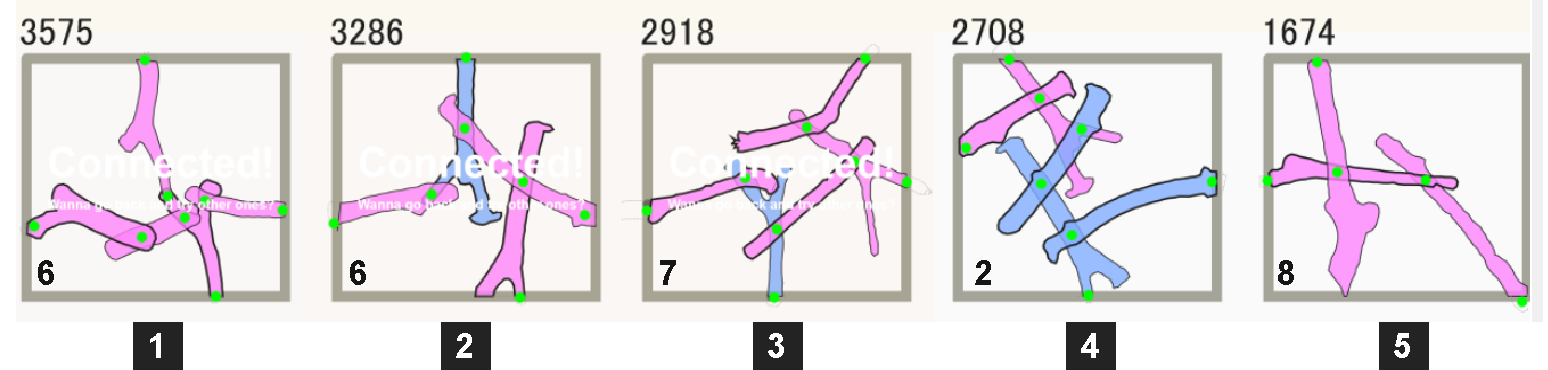
\includegraphics[width = 0.4\paperwidth]{images/fabrication/casestudy.pdf}
		\caption{The five completed layouts by participants. The number on top left indicates each score, and the bottom left is the frame number (see also Figure 1 right top).   }
		\label{fig:layouts}
	\end{center}
\end{figure}

\subsubsection*{Fabrication}
We observed most of scanned models had occluded regions between plates and branches, which created interpolated faces after surface reconstruction by iSense application, resulting in outwardly offsetted contours. After milling was finished and when branches were assembled, six pairs of branches were loosely connected because the calculated contours were 2-3 $mm$ eroded than the actual sizes.
We avoided this problem by trimming branches from 2-5 $mm$ higher than the plate surface.
After this operation, the rest of connections were tightly connected. \\

We also observed that many milling paths were 5-10 $mm$ off from where they were planned.
Multiple reasons could be considered as follows: 1. deformation of mechanical parts of the CNC router. 2. not dense resolution of acquired contours of branches. 3. misaligned orientation of the plate compared to the scanned model.
To avoid the misalignments, we modified the \textit{G-Code Generator} so that an operator can freely adjust the absolute origin of generated milling paths per plate.
Before the modification, an origin was set at the bottom left corner of plates.
After the modification, it became easier to reset the origin in case of large misalignments, however, the origin set at the center of plate was good enough for our purpose.
After this modification, misalignments stayed within 3 $mm$.
Branches could absorb 3-5 $mm$ misaligned joint positions due to the elasticity of branches, which also solidifies the structure.
 % with residual stresses from the misalignments.
% The misaligned joint positions worked as post-tensions, solidifying the structure.
% We assume that this is only applicable when an applied bending moment and cut surface at a joint is orthogonal or not too much off from orthogonal. \todo{this sentence}

\section{Conclusion}
% \subsubsection*{Summary}
In this paper, we presented a workflow to design and fabricate with branches in their native forms, which are not large enough to be used as standardized building components.
Our workflow was validated by the case study with lower-aged participants without design and fabrication experiences.

Our online platform with stored scanned branches and the game is accessible.
Multiple users can submit design layouts and explore a global design. % and locations.
Our branch joint and group condition update algorithms are running on the browser game which can be accessed from laptops and mobile devices, contributing to the accessibility of the presented workflow.
Together with the accessibility, the intuitive interface was simple for non-expert users, validated by the case study.
We successfully built a network of branches with rigid joints generated by our joint milling path generator.
Each of joints has customized lapped-joint geometry, which extends design possibilities of branches or woods in native forms.

% \subsubsection*{Limitations and Future Work}
Our workflow consists of many technological components such as skeleton extraction, structural optimization, object detection/recognition, and data-driven design-fabrication.
Focusing on the use of native forms, each step of our workflow has potential to contribute to each area with the use of native forms of natural materials.
Also, our workflow was developed based on the participation of users, thus the entire process is not necessarily automated, however, some tasks could be improved to assist users.

The skeleton extraction could take incomplete point-set directly from original tree branches before they are cut in length.
With data-driven approach, the system could distinguish trees and which part of tree the branch from.
With morphological analysis, the system could suggest users where to cut branches to achieve user-defined target design.
Structural and geometrical validity/invalidity of obtained materials could be analyzed.
Our workflow requires branches to be fixed on a plate, which takes the longest duration in the workflow except for in-between tasks such as moving and pausing.
Using a robotic manipulator with a gripper, the attaching process could be skipped.

Our game system is limited in 2D, whereas original branch forms have rich 3D geometry with textures.
In our case, these information was used in limited ways such as in skeleton extractions and G-Code generation.
Despite of successfully fabricated non-orthogonal joints, we did not complete the attaching branches to the target frames, as we prioritized to validate branch-branch joints.
Our layout design process is fully dependent on users with limited feedback during design process.
The game can provide suggestive feedback with structural analysis of each joint and entire structure.
% As the problem of limited number of branches and fixed target points to be connected, the system could assist humans to reach to structurally sound solutions with less efforts.

% The performance of our joint detection and alalgorithm could be
Our joint and group detection algorithms are limited with materials with skeletons, and our joint generator is limited to branches.
Both steps use down-sampled or high-resolution point sets.
It is valuable to validate the approach by comparing with other available methods such as collision detections or joint detection with down-sampled model by interpolation.

Finally, our game-based design could be applied to different purposes, not only for participatory layout design but also for collecting data of user behaviors during design.
Also application to other kinds of materials could be investigated.


%\section*{Acknowledgments}
%We appreciate the public house for hosting the CNC router and providing participants for the user study.
%We thank to the film editor, Shin Yamane for shooting our video clips.
%We also thank to the developer of an online game \textit{2048}, Gabriele Cirulli and his contributors, for sharing source code in Github community.


\bibliographystyle{acmsiggraph}
\nocite{*}
\bibliography{references}


 \appendix
 \section{Group Update process}
 The group update process is described as follows.
 Each time the process is called, firstly it initializes a set of groups denoted as $\mathcal{G}$.
 Iterating $b_i \in \mathcal{B}$, the first group $g_0 \in \mathcal{G}$ is created and $g_0$ stores $b_0$.
 In the iteration, the process checks connections of a branch $b_i$ with all the existing groups $ g_j \in \mathcal{G}$.
 If $b_i$ is connected to $g_j$, $g_j$ is stored in a list of connected groups, denoted as $C_i$.
 After collecting all the connected groups with $b_i$, we evaluates $C_i$.
 If $C_i$ does not have any stored group, then a new group $g$ storing $b_i$ is created and added to $\mathcal{G}$.
 If $C_i$ is not empty, then it also creates a new group $g$, but puts all the groups $g_j \in C_i$ to $g$, then adds $g$ to $\mathcal{G}$.
 Finally groups $g_j \in C_i$ are removed from $\mathcal{G}$.
 Iterating all $b_i \in \mathcal{B}$, we acquire the updated group condition.

 \begin{algorithm}
   \caption{Group Condition Update Algorithm}
   \begin{algorithmic}[1]
     \Function{UpdateGroups}{$\mathcal{B}$}
     \State{Reset all the groups $\mathcal{G}$ }
     \State{Create new group $g_0$}
     \State{$g_0$.adds $\left( b_0 \right) $}
 %    \If{$b_0$.contains$\left( t_i \in \mathcal{T} \right) $ }
 %      \State{$g_0$.adds$\left(t_i \right) $}
 %    \EndIf
     \State{$\mathcal{G}$.adds$\left( g_0 \right) $ }

     \For{each branch $b_i \in \mathcal{B}$ except $b_0$}
     \State{\textit{initiate a list of connected group} $C_i$}
       \For{each group $g_j \in \mathcal{G}$}
           \If{ $g_j$.isConnectedTo$ \left( b_i \right)$}
             \State{ $C_i$.add$\left( g_j \right) $}
           \EndIf
       \EndFor

   	\State{Create new group $g$}
 	% \If{$C_i$.hasMember}
 		\For{each group $g_j \in  C_i$}
 			\For{each branch $b_k \in g_j$}
 %				\If{$g$.contains$\left( b_k \right) =false$}
 						\State{$g$.adds$\left(b_k \right) $}
 %				\EndIf
 			\EndFor
 		\EndFor
 		\For{each group $g_j \in  C_i$}
 			\State{$\mathcal{G}$.removes$\left(g_j \right) $}
 		\EndFor
 	% \EndIf
 	\State{$g$.adds$\left(b_i \right) $}
 	\State{$\mathcal{G}$.adds$\left( g \right) $ }
 	\EndFor
   \EndFunction
   \end{algorithmic}
   \label{al:connection}
 \end{algorithm}

\end{document}
